% You can define macros here

\title{The best EAGE abstract of all time}
\author{Jeff Godwin and Friends, Center for Wave Phenomena, Colorado School of Mines}

\maketitle

\section{Introduction}

Lorem ipsum dolor sit amet, consectetur adipiscing elit. Donec lacus urna, porta nec facilisis eget, ultricies non purus. Donec dui leo, vestibulum ut rutrum in, fringilla sit amet dui. Sed cursus, nunc ac congue varius, ante nisi commodo velit, ut auctor lorem magna nec neque. Vivamus et tempor augue. Sed vulputate congue nulla, non feugiat dolor auctor a. Etiam lectus diam, fringilla at adipiscing non, blandit sit amet nunc. Donec tincidunt, erat id molestie tincidunt, libero ligula facilisis tellus, ac cursus justo nulla sed magna. Aenean arcu mi, fermentum eu mattis ut, scelerisque sit amet sem. Cras vitae dictum felis. Ut ut ante fermentum metus posuere consectetur at sed ligula. Maecenas eget ante et lorem dignissim pretium. Curabitur quam sem, malesuada a porta quis, rhoncus ut dui. Ut malesuada sapien in lectus lobortis molestie. Sed non tellus tincidunt ligula congue convallis et auctor dolor.

\section{Theory}
Morbi porttitor, tortor eu pulvinar luctus, nisl mi placerat sem, id iaculis lacus ipsum at urna. Vivamus adipiscing semper sem placerat volutpat. Proin luctus mattis pulvinar. Vivamus auctor dui vel odio vestibulum in convallis lacus vehicula. Vivamus nec leo libero. Nam eu neque in massa posuere congue nec ut neque. Nullam et tortor dolor, a scelerisque diam. Sed pulvinar neque vitae lorem cursus eget laoreet lacus tempus. Phasellus dapibus, mi porttitor dignissim rhoncus, mauris nisi egestas dui, sed laoreet risus dolor quis dolor. Vivamus et elit sapien, non vulputate metus. Vivamus risus lorem, tristique nec tristique ac, iaculis elementum lacus. Sed id libero porttitor diam mollis iaculis. Vestibulum eget nisi non ante fringilla rutrum. Nam nibh nisi, convallis at tincidunt a, elementum vitae enim. Quisque sit amet tincidunt dolor.

\section{Demonstration}
Here's a short demo of how to use some common features inside of the provided \LaTeX classes.

Equations:
\begin{equation}
    \nabla^2 u - \alpha \frac{\partial u}{\partial t} = 0
\label{eqn:demo}
\end{equation}

Here is how we use equations: ~\ref{eqn:demo}.  Here is how we can make citations \cite[]{godwin_blended_2010,krebs_fast_2009,duquet_3d_1999}. Or we can cite inline as in \cite{godwin_blended_2010}.

We can also make figures using our Madagascar plots.  There are two ways to do so, 1 - using built-in macros and 2 - using the default \LaTeX macros.

The first way:
\plot{Fig1}{width=0.45\textwidth}{A plot of our signal.}
\sideplot{Fig2}{width=0.45\textwidth}{The amplitude spectrum of our signal.}

\multiplot{2}{Fig1,Fig2}{width=0.45\textwidth}{The signal (a), and the amplitude spectrum (b) plotted using multiplot (which is great for making large plots across columns).}


Or we could use includegraphics as usual:

\begin{figure}
    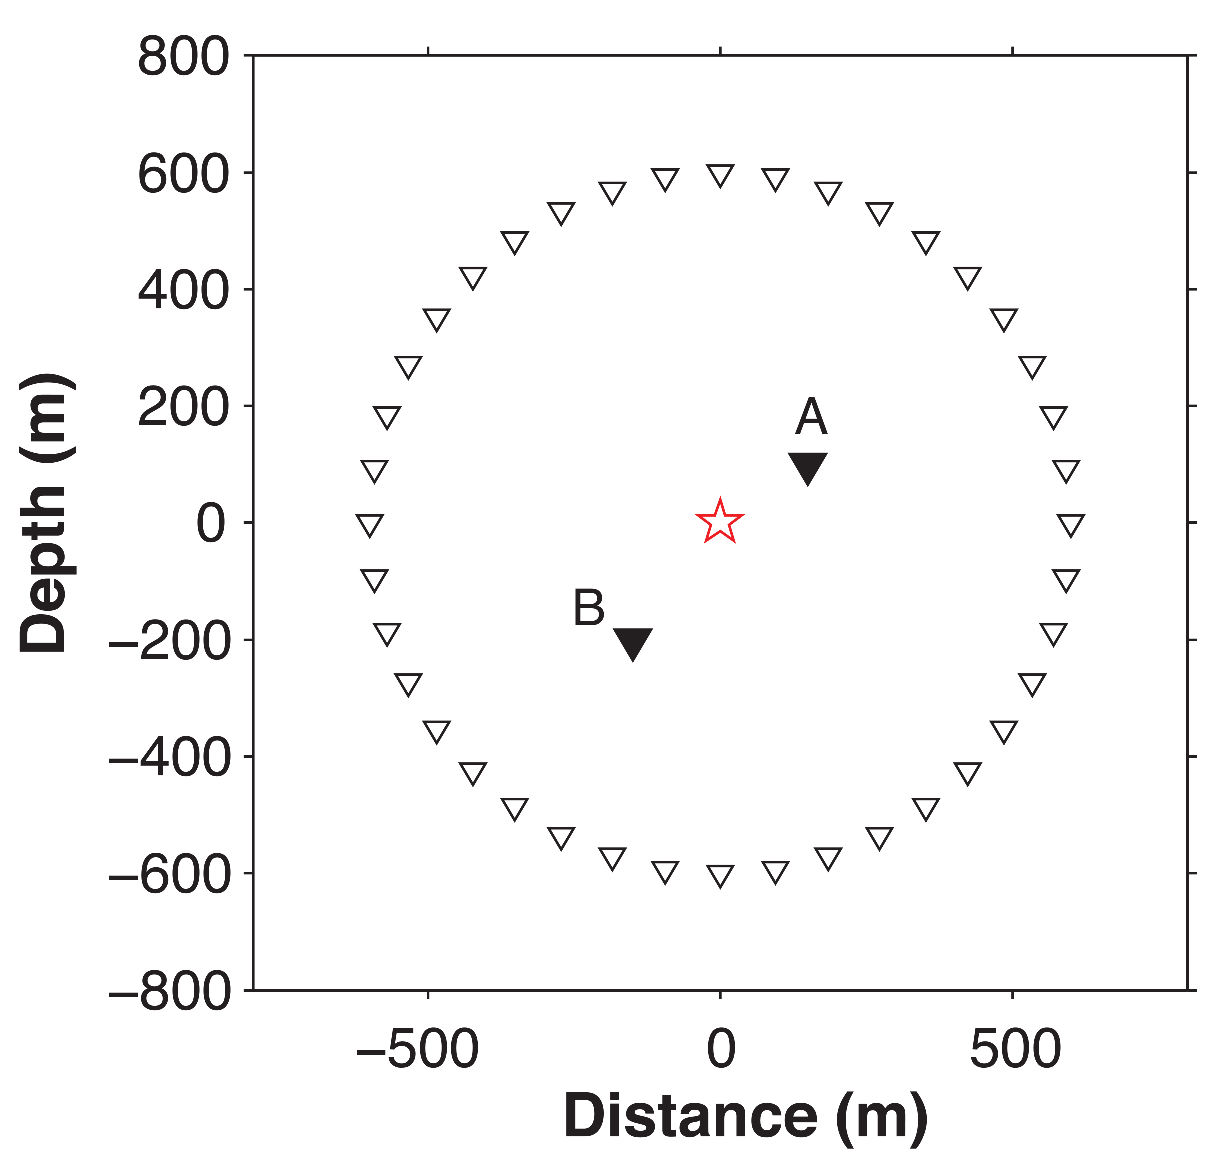
\includegraphics[width=0.45\textwidth]{Fig/Fig1} 
    \caption{The signal.}
\label{Fig:noise}
\end{figure}

To reference figures we use Figure~\ref{fig:noise}, or we can use, Figures~\ref{fig:noise}-~\ref{fig:spectra}. Note, the example here has bad numbering because we plot the same figure multiple times which confuses \LaTeX.  No normal paper would plot the same figure multiple times, and numbering would be correct.

We can also use any other \LaTeX commands as usual.  You just have to include the correct packages in your SConstruct.

\section{Results}

Sed vitae elit neque. Pellentesque habitant morbi tristique senectus et netus et malesuada fames ac turpis egestas. Phasellus rhoncus, augue in egestas egestas, elit neque tempor diam, eget vulputate nisi odio sit amet neque. Vestibulum ante ipsum primis in faucibus orci luctus et ultrices posuere cubilia Curae; In scelerisque lectus a est gravida ut blandit nunc condimentum. Nam faucibus eros sit amet mauris fringilla fermentum. Donec vel odio urna. Nunc sit amet nibh sed tortor volutpat tincidunt. Lorem ipsum dolor sit amet, consectetur adipiscing elit. Ut dui tortor, egestas sit amet scelerisque porta, tempus ut nulla. Cras aliquam ornare luctus. Etiam condimentum orci eu odio luctus aliquet. Vestibulum commodo faucibus nulla, in feugiat velit tincidunt et. In consequat placerat ligula quis lacinia.

\section{Conclusions}

Nulla ultricies convallis massa, et rutrum nisi dictum a. Donec id ligula in arcu adipiscing eleifend vel sed erat. Nulla et urna at purus accumsan pharetra ac vel enim. Sed metus nunc, dictum non facilisis quis, ullamcorper eu lorem. Curabitur congue porttitor orci, ut accumsan dui tincidunt non. Aliquam metus urna, faucibus sed posuere eget, pharetra id est. Nunc in nisi eget dolor tempus accumsan a condimentum dolor. Sed est dui, varius quis tempus sodales, egestas et odio. Ut aliquet ullamcorper neque in condimentum.

Ut auctor, purus et cursus euismod, sapien purus tempor libero, ac commodo tellus nulla quis dolor. Vivamus quis enim mauris. Duis magna lorem, ullamcorper nec porttitor ac, commodo quis turpis. In ornare auctor dui, sit amet auctor massa congue porttitor. Nam pellentesque arcu at lectus luctus sit amet dictum nisl tempor. Sed lobortis nisi in eros vulputate ac ullamcorper felis pharetra. Praesent lorem neque, egestas ac ultricies a, adipiscing feugiat eros. Curabitur id quam id ante consectetur porta. Sed imperdiet nibh eget tellus imperdiet sed varius arcu euismod. Nunc egestas arcu sed mauris molestie sollicitudin. Cras convallis gravida sodales. Praesent venenatis, diam vitae gravida sollicitudin, ante diam lobortis erat, vel consectetur turpis nisi sed mauris. Cras nec sem mauris, eu lacinia quam. Nullam at quam lorem, quis dignissim ligula.

\bibliographystyle{seg}
\bibliography{demobib}
